\begin{figure}[ht]
\centering
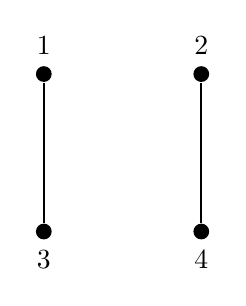
\begin{tikzpicture}[
       thick,
       acteur/.style={
         circle,
         fill=black,
         thick,
         inner sep=2pt,
         minimum size=0.2cm
       }
     ]

       \node (a1) at (0,0) [acteur,label=below:3]{};
       \node (a2) at (0,2)[acteur,label=above:1]{}; 
       \node (a3) at (2,2) [acteur,label=above:2]{}; 
       \node (a4) at (2,0) [acteur,label=below:4]{}; 
  
       \draw (a1) -- (a2); 
       \draw (a3) -- (a4); 

\end{tikzpicture}
  \caption{The support of a $1$-cosystole, which can not be determined using disjoint cycles}
\end{figure}
